%Version 3.1 December 2024
% See section 11 of the User Manual for version history
%
%%%%%%%%%%%%%%%%%%%%%%%%%%%%%%%%%%%%%%%%%%%%%%%%%%%%%%%%%%%%%%%%%%%%%%
%%                                                                 %%
%% Please do not use \input{...} to include other tex files.       %%
%% Submit your LaTeX manuscript as one .tex document.              %%
%%                                                                 %%
%% All additional figures and files should be attached             %%
%% separately and not embedded in the \TeX\ document itself.       %%
%%                                                                 %%
%%%%%%%%%%%%%%%%%%%%%%%%%%%%%%%%%%%%%%%%%%%%%%%%%%%%%%%%%%%%%%%%%%%%%

%%\documentclass[referee,sn-basic]{sn-jnl}% referee option is meant for double line spacing

%%=======================================================%%
%% to print line numbers in the margin use lineno option %%
%%=======================================================%%

%%\documentclass[lineno,pdflatex,sn-basic]{sn-jnl}% Basic Springer Nature Reference Style/Chemistry Reference Style

%%=========================================================================================%%
%% the documentclass is set to pdflatex as default. You can delete it if not appropriate.  %%
%%=========================================================================================%%

%%\documentclass[sn-basic]{sn-jnl}% Basic Springer Nature Reference Style/Chemistry Reference Style

%%Note: the following reference styles support Namedate and Numbered referencing. By default the style follows the most common style. To switch between the options you can add or remove “Numbered” in the optional parenthesis. 
%%The option is available for: sn-basic.bst, sn-chicago.bst%  
 
%%\documentclass[pdflatex,sn-nature]{sn-jnl}% Style for submissions to Nature Portfolio journals
%%\documentclass[pdflatex,sn-basic]{sn-jnl}% Basic Springer Nature Reference Style/Chemistry Reference Style
\documentclass[pdflatex,sn-mathphys-num]{sn-jnl}% Math and Physical Sciences Numbered Reference Style
%%\documentclass[pdflatex,sn-mathphys-ay]{sn-jnl}% Math and Physical Sciences Author Year Reference Style
%%\documentclass[pdflatex,sn-aps]{sn-jnl}% American Physical Society (APS) Reference Style
%%\documentclass[pdflatex,sn-vancouver-num]{sn-jnl}% Vancouver Numbered Reference Style
%%\documentclass[pdflatex,sn-vancouver-ay]{sn-jnl}% Vancouver Author Year Reference Style
%%\documentclass[pdflatex,sn-apa]{sn-jnl}% APA Reference Style
%%\documentclass[pdflatex,sn-chicago]{sn-jnl}% Chicago-based Humanities Reference Style

%%%% Standard Packages
%%<additional latex packages if required can be included here>

\usepackage{graphicx}%
\usepackage{multirow}%
\usepackage{amsmath,amssymb,amsfonts}%
\usepackage{amsthm}%
\usepackage[title]{appendix}%
\usepackage{xcolor}%
\usepackage{textcomp}%
\usepackage{manyfoot}%
\usepackage{booktabs}%
\usepackage{url}
\usepackage{algorithm}%
\usepackage{algorithmicx}%
\usepackage{algpseudocode}%
\usepackage{listings}
\usepackage[utf8]{inputenc}
\usepackage[T1]{fontenc}
%%%%

%%%%%=============================================================================%%%%
%%%%  Remarks: This template is provided to aid authors with the preparation
%%%%  of original research articles intended for submission to journals published 
%%%%  by Springer Nature. The guidance has been prepared in partnership with 
%%%%  production teams to conform to Springer Nature technical requirements. 
%%%%  Editorial and presentation requirements differ among journal portfolios and 
%%%%  research disciplines. You may find sections in this template are irrelevant 
%%%%  to your work and are empowered to omit any such section if allowed by the 
%%%%  journal you intend to submit to. The submission guidelines and policies 
%%%%  of the journal take precedence. A detailed User Manual is available in the 
%%%%  template package for technical guidance.
%%%%%=============================================================================%%%%

%% as per the requirement new theorem styles can be included as shown below
\theoremstyle{thmstyleone}%
\newtheorem{theorem}{Theorem}%  meant for continuous numbers
%%\newtheorem{theorem}{Theorem}[section]% meant for sectionwise numbers
%% optional argument [theorem] produces theorem numbering sequence instead of independent numbers for Proposition
\newtheorem{proposition}[theorem]{Proposition}% 
%%\newtheorem{proposition}{Proposition}% to get separate numbers for theorem and proposition etc.

\theoremstyle{thmstyletwo}%
\newtheorem{example}{Example}%
\newtheorem{remark}{Remark}%

\theoremstyle{thmstylethree}%
\newtheorem{definition}{Definition}%

\raggedbottom
%%\unnumbered% uncomment this for unnumbered level heads

\begin{document}

\title[Article Title]{Automated Fine-Tuning of Diffusion Models for Learning Underrepresented Concepts from Web-Scraped Data}

%%=============================================================%%
%% GivenName	-> \fnm{Joergen W.}
%% Particle	-> \spfx{van der} -> surname prefix
%% FamilyName	-> \sur{Ploeg}
%% Suffix	-> \sfx{IV}
%% \author*[1,2]{\fnm{Joergen W.} \spfx{van der} \sur{Ploeg} 
%%  \sfx{IV}}\email{iauthor@gmail.com}
%%=============================================================%%

\author*[1]{\fnm{Felipe} \sur{Mahlow}}\email{f.mahlow@unesp.br}

\author[1]{\fnm{Renato} \sur{Dias de Souza}}\email{renato.dias@unesp.br}


\author[1]{\fnm{João Paulo} \sur{Papa}}\email{joao.papa@unesp.br}


\author[1]{\fnm{Kelton Augusto} \sur{Pontara da Costa}}\email{kelton.costa@unesp.br}


\affil*[1]{\orgdiv{Faculty of Sciences}, \orgname{Sao Paulo State University}, \orgaddress{\street{Av. Eng. Luís Edmundo Carrijo Coube, 14-01}, \city{Bauru}, \postcode{17033-360}, \state{SP}, \country{Brazil}}}


%%==================================%%
%% Sample for unstructured abstract %%
%%==================================%%

\abstract{Despite significant advancements in image generation models, they still struggle to accurately depict culturally specific concepts, such as regional languages, landscapes, mythology, and artistic traditions. While these models excel at generating common objects, they often lack the necessary adaptability to represent nuanced cultural elements. This paper introduces an automated pipeline that streamlines the fine-tuning process, enabling the customization of generative models for user-defined prompts. \textcolor{blue}{The pipeline integrates web scraping with a human-in-the-loop curation interface, DreamBooth-style LoRA fine-tuning of Stable Diffusion XL, and Latent Consistency Model inference. We evaluate it on eight culturally specific concepts from three categories (foods, folklore beings, and artifacts/clothing), each learned from 20 human-verified images, using CLIP Score, FID, and KID over 1000 generated images per condition. After fine-tuning, the CLIP Score increased for every concept, by 6.8 to 15.5 points, and FID decreased for every concept. Under matched data and generation settings, the pipeline also outperformed a Textual Inversion baseline in CLIP Score and FID for all eight concepts. A qualitative analysis shows that the composition of the few training images can still introduce cultural misreadings, which motivates careful curation. We derive practical guidelines on dataset composition, training duration, and evaluation.}}

%%================================%%
%% Sample for structured abstract %%
%%================================%%

% \abstract{\textbf{Purpose:} The abstract serves both as a general introduction to the topic and as a brief, non-technical summary of the main results and their implications. The abstract must not include subheadings (unless expressly permitted in the journal's Instructions to Authors), equations or citations. As a guide the abstract should not exceed 200 words. Most journals do not set a hard limit however authors are advised to check the author instructions for the journal they are submitting to.
% 
% \textbf{Methods:} The abstract serves both as a general introduction to the topic and as a brief, non-technical summary of the main results and their implications. The abstract must not include subheadings (unless expressly permitted in the journal's Instructions to Authors), equations or citations. As a guide the abstract should not exceed 200 words. Most journals do not set a hard limit however authors are advised to check the author instructions for the journal they are submitting to.
% 
% \textbf{Results:} The abstract serves both as a general introduction to the topic and as a brief, non-technical summary of the main results and their implications. The abstract must not include subheadings (unless expressly permitted in the journal's Instructions to Authors), equations or citations. As a guide the abstract should not exceed 200 words. Most journals do not set a hard limit however authors are advised to check the author instructions for the journal they are submitting to.
% 
% \textbf{Conclusion:} The abstract serves both as a general introduction to the topic and as a brief, non-technical summary of the main results and their implications. The abstract must not include subheadings (unless expressly permitted in the journal's Instructions to Authors), equations or citations. As a guide the abstract should not exceed 200 words. Most journals do not set a hard limit however authors are advised to check the author instructions for the journal they are submitting to.}

\keywords{Text-to-Image Diffusion Models, Few-Shot Fine-Tuning, \textcolor{blue}{Cultural Representation}, Image Synthesis}

%%\pacs[JEL Classification]{D8, H51}

%%\pacs[MSC Classification]{35A01, 65L10, 65L12, 65L20, 65L70}

\maketitle

\section{Introduction}\label{sec1}

Recent advancements in generative models, such as diffusion-based models and Generative Adversarial Networks (GANs)~\cite{goodfellow2014generativeadversarialnetworks}, have significantly improved the quality and flexibility of image generation. A particularly efficient variation, Latent Diffusion Models (LDMs)~\cite{rombach2022high}, operates in a compressed latent space, optimizing computational efficiency while maintaining visual realism. Among the most notable image generation models are DALL-E~\cite{betker2023improving}, \textcolor{blue}{Midjourney}\footnote{\url{https://www.midjourney.com/home}}, and Stable Diffusion~\cite{rombach2022high}, which leverage sophisticated attention mechanisms and latent representations to synthesize highly detailed images. Concurrently, GANs~\cite{goodfellow2016deep} continue to play a crucial role in generating high-fidelity images by utilizing an adversarial framework in which a generator and a discriminator compete to refine image quality.  

Despite these technological advancements, generative models are trained on large-scale datasets that often reflect societal biases and fail to adequately represent less common or culturally specific concepts~\cite{navigli2023biases}. Many datasets used for training are predominantly composed of Western-centric imagery, leading to a lack of diversity in the generated outputs~\cite{NEURIPS2024_18c669b8}. Consequently, these models struggle to accurately depict regional languages, landscapes, mythology, and cultural artifacts~\cite{pampas}. This limitation not only affects the accuracy of generated images but also reinforces existing imbalances in digital representation.  Given the widespread adoption of AI-generated imagery, it becomes essential to develop strategies that mitigate biases and promote a more inclusive representation of underrepresented concepts~\cite{sci6010003}. Addressing these disparities is crucial for enhancing the applicability of generative AI in fields that demand cultural sensitivity, such as historical preservation, education, and digital art. 

Fine-tuning techniques have emerged as a powerful solution, enabling models to adapt to new concepts using smaller, domain-specific datasets. Among existing fine-tuning methods, DreamBooth~\cite{dreambooth} and Textual Inversion~\cite{textualinversion} have demonstrated significant potential for teaching generative models new visual concepts. These approaches enable models to generate images of specific objects, styles, or subjects with minimal training data. However, fine-tuning a model manually remains a time-consuming and computationally expensive process, requiring expertise in dataset curation and model optimization.  

To overcome these challenges, this paper proposes an automated pipeline for fine-tuning a text-to-image diffusion model, enabling users to efficiently teach models new concepts with minimal manual intervention. Our approach integrates web scraping—a technique for automatically gathering images from the internet—combined with fine-tuning strategies such as Low-Rank Adaptation (LoRA)~\cite{hu2021loralowrankadaptationlarge}. LoRA reduces the number of trainable parameters in the model, making fine-tuning more efficient while preserving the original model's generalization capabilities. Additionally, we utilize Latent Consistency Models (LCMs)~\cite{luo2023latent} to accelerate the image generation process, significantly reducing the number of inference steps required to produce high-quality outputs. By automating both dataset collection and model fine-tuning, we aim to make generative AI more accessible and customizable for diverse applications.  

Our study focuses on fine-tuning generative models to learn concepts that are underrepresented in large-scale datasets, particularly culturally specific elements that mainstream models struggle to depict accurately. To evaluate the effectiveness of our approach, we selected eight distinct cultural concepts from various countries, \textcolor{blue}{spanning three categories: foods, folklore and mythological beings, and artifacts, clothing, and objects.} These concepts serve as test cases for assessing how well our fine-tuned models can generate images \textcolor{blue}{that capture the key visual attributes of each concept, and how fine-tuning affects} the inherent biases present in pre-trained generative models. Our evaluation process consisted of both qualitative and quantitative analyses. First, we conducted a qualitative assessment to identify biases present in the base model and analyze the patterns observed before and after fine-tuning. This step allowed us to examine common distortions, omissions, or misrepresentations of culturally specific elements, providing insights into how the model initially struggled with underrepresented concepts and how fine-tuning influenced its generative behavior.

To complement this analysis, we employed quantitative metrics to systematically measure improvements during fine-tuning. Specifically, we used CLIP Score~\cite{hessel2021clipscore} to evaluate the semantic alignment between generated images and their corresponding textual descriptions, ensuring that the model effectively captured the intended cultural concepts. Additionally, we computed the Fréchet Inception Distance (FID)~\cite{heusel2018ganstrainedtimescaleupdate} to assess the visual quality and diversity of the generated images by comparing their feature distributions with those of real images from our dataset. By tracking these metrics throughout the training process, we ensured that fine-tuning led to meaningful improvements in both semantic coherence and image fidelity. \textcolor{blue}{Because FID is unreliable when the set of real images is small, we also report the Kernel Inception Distance (KID).} We further investigate the impact of training duration on fine-tuning effectiveness, analyzing the \textcolor{blue}{number of steps required for models to learn underrepresented concepts. Our checkpoint-wise experiments show that more than half of the final CLIP Score gain is already reached after $1000$ training steps for every concept, while training up to $3000$ steps still brings smaller additional gains, which lets users trade computational cost against performance.}


\textbf{Main Contributions}: This paper presents an automated framework for fine-tuning text-to-image diffusion models using web-scraped datasets \textcolor{blue}{ combined with a lightweight human-in-the-loop curation step, substantially reducing the effort required for manual data collection.} We assess the models' effectiveness in generating images of underrepresented concepts using qualitative and quantitative metrics\textcolor{blue}{, including CLIP Score, FID, and, to complement FID under a small reference set, the Kernel Inception Distance (KID), each reported with bootstrap confidence intervals over 1000 generated images per condition}. \textcolor{blue}{We also analyze how the metrics evolve across training checkpoints, providing guidance on the choice of training duration to balance computational cost and performance, and we compare our DreamBooth+LoRA pipeline against a Textual Inversion baseline under matched data and generation settings.} Latent Consistency Models (LCMs) are integrated to reduce the computational demands of high-quality image generation. Additionally, we explore biases in generative models, outlining their limitations and suggesting ways to improve cultural representation.

This paper is structured as follows: Section~\ref{related_work} \textcolor{blue}{reviews related work on generative models and fine-tuning techniques.} Section~\ref{methods} presents the methodology, detailing the web scraping process, dataset collection, model fine-tuning, inference pipeline with LCMs, and the metrics utilized. Section~\ref{results} discusses the experimental results, both from a qualitative and quantitative perspective. Finally, Section~\ref{conclusions} concludes the paper by summarizing key findings, evaluating the effectiveness of the proposed pipeline, and outlining potential directions for future research. 

\section{Related Work}
\label{related_work}

\textbf{Diffusion Models:} One of the most notable examples is Stable Diffusion~\cite{rombach2022high}, where the diffusion process takes place in the latent space instead of the pixel space. In this architecture, text embeddings from a pre-trained CLIP~\cite{clip} model are fed into a UNet enhanced with cross-attention. Stable Diffusion XL~\cite{sdxl} further improves upon this by incorporating a more robust UNet and a larger CLIP text encoder, refining text-to-image conditioning. Other models, such as DALL-E 3~\cite{betker2023improving}, achieve comparable results by using enhanced synthetic captions to boost CLIP Score performance. The recent FLUX.1 Kontext~\cite{labs2025flux1kontextflowmatching} presents a flow‐matching model that unifies image generation and editing in latent space, achieving high consistency across multiple iterations and interactive speeds. The Diffusion Visual Programmer (DVP)~\cite{han2024imagetranslationdiffusionvisual} is a neuro-symbolic image translation framework that incorporates a conditionally flexible diffusion model with GPT-based visual programming to perform “where-then-what” edits in a controllable, explainable, and high-fidelity manner.

In video, diffusion models with a 3D causal VAE and an expert transformer (CogVideoX)~\cite{yang2025cogvideoxtexttovideodiffusionmodels} produce long-duration (up to 10 s at 16 fps and 768×1360) coherent, semantically aligned, high-fidelity videos, achieving state-of-the-art performance. And for text-to-video retrieval, DITS~\cite{NEURIPS2024_0731f0e6} is a diffusion-inspired truncated sampler that progressively aligns text and video embeddings with a contrastive loss to model the multimodal gap, achieving state-of-the-art text-video retrieval performance.


\textbf{Fine-tuning:} Alongside the advancements in large-scale architectures, fine-tuning techniques have gained prominence for adapting text-to-image models to specific domains or personalized subjects. DreamBooth~\cite{dreambooth} and Textual Inversion~\cite{textualinversion} are particularly effective in few-shot scenarios, enabling personalized generation from very limited samples. New approaches such as Specialist Diffusion~\cite{Specialist-Diffusion} and Object-Driven One-Shot Fine-Tuning with Prototypical Embedding~\cite{lu2024object} aim to further reduce overfitting and improve fidelity. These methods facilitate adaptation to novel objects, styles, and even cultural elements via specialized fine-tuning strategies. In Large Language Models (LLMs), APROMPT~\cite{wang2023aprompt} introduces trainable query, key, and value prompts directly into the attention mechanism—beyond traditional input-level prompt tuning—enabling efficient and highly effective fine-tuning with fewer parameters.




%\textbf{Other methods:} Recently, various techniques have been proposed to enhance the control and quality of diffusion models in the image generation process. Among these, adapters stand out, enabling the incorporation of additional conditional controls, as demonstrated by Zhang et al. (2023)~\cite{zhang2023adding}, who introduced adapters for text-to-image diffusion models, allowing for more precise manipulation of generated outputs. Another relevant approach is compositional generation, explored by Du et al. (2023)~\cite{du2023reduce} and Liu et al. (2022)~\cite{liu2022compositional}, which combines multiple diffusion models or employs energy-based techniques to create images with greater complexity and quality. Additionally, classifier-based guidance, proposed by Dhariwal and Nichol (2021)~\cite{dhariwal2021diffusion}, has proven effective in improving the fidelity of generated images, while classifier-free guidance, introduced by Ho and Salimans (2021)~\cite{ho2022classifier}, offers greater autonomy in the generation process, aligning outputs more closely with user intentions. These approaches have significantly contributed to the advancement of diffusion models, enabling greater control and quality in image generation applications.

While the methods discussed above are highly impactful in their respective areas, our approach stands out for its accessibility and cultural focus. Unlike previous techniques that require technical expertise, our pipeline automates dataset creation and fine-tuning, making it usable even by non-experts. Moreover, by targeting niche applications and cultural preservation, our method enables the integration of underrepresented visual identities. This expands the inclusivity and contextual relevance of generative models, allowing them to reflect a broader spectrum of human creativity.

\section{Methodology}
\label{methods}

This section details the methodology employed to develop and implement the pipeline. The methodology comprises multiple stages, including image scraping, model training, and image generation, facilitated by a web-based user interface. Additionally, we present the criteria used for \textcolor{blue}{selecting the concepts that serve as test cases} in our study and, finally, provide the theoretical foundation necessary to understand the metrics used for evaluation.

\paragraph*{\textcolor{blue}{Role of LoRA and LCM in our system.}}
\textcolor{blue}{We emphasize that our contribution is primarily a systems and methodology pipeline focused on automation, reproducibility, and cultural applicability, rather than on proposing new model architectures. In this pipeline, \emph{training-time} concept adaptation is performed through LoRA fine-tuning (Section~\ref{sec:training}), whereas \emph{inference-time} acceleration is achieved via Latent Consistency Model (LCM) scheduling (Section~\ref{sec:generation}), enabling high-quality generations with substantially fewer sampling steps.}


\subsection{Image Scraping}

Web scraping is a fundamental technique for collecting visual data, playing a crucial role in building datasets and enhancing machine learning models, particularly generative ones. By automating the retrieval of images from the web, this process enables the efficient and scalable acquisition of diverse visual content. In this study, we employ a Selenium-based web scraper to navigate Google Images and extract a specified number of images based on predefined concepts, streamlining dataset construction.

The process begins with the initialization of a headless Chrome browser instance, which is used to perform the search without a visible user interface. The browser navigates to Google Images and executes a search query for the specified concept. Once the search results are loaded, the script iterates through the retrieved images, extracting their URLs. Depending on the format, images are either decoded from \textit{base64} encoding or downloaded directly via HTTP requests. \textcolor{blue}{For each cultural concept, we used a fixed training set of \textbf{20 images}. This choice is intentional and aligned with the DreamBooth paradigm, which is specifically designed to learn new concepts from extremely small datasets. By operating in a few-shot regime, the fine-tuning process significantly reduces the burden of dataset collection and makes manual curation feasible and effective. In culturally sensitive scenarios, this is particularly important, as it allows users to carefully inspect and filter each sample, minimizing noise and reducing the risk of introducing biased or misleading representations during training.
} \textcolor{blue}{Since each fine-tuning run targets a single concept with only a few images, conventional dataset balancing or re-weighting strategies, which assume larger datasets with multiple classes or demographic groups, are not directly applicable. In this regime, bias control is instead exercised through the careful selection of each training image, for instance, by ensuring that the samples depict the concept in its appropriate cultural context and cover its relevant visual variations.}

After retrieval, the images are processed to ensure consistency. Each image is converted to the RGB format if necessary and resized to maintain uniformity across the dataset. Finally, the processed images are systematically stored in a designated 	output folder, preserving their structure for further use in model training and evaluation. This automated approach enables the rapid collection of concept-specific images, facilitating their integration into machine learning pipelines.

We emphasize that the central contribution of this work is the automated, human-guided workflow for dataset construction and fine-tuning, rather than a dependence on any specific image source. While our reference implementation uses Google Images for convenience, the same pipeline can be straightforwardly adapted to ingest images from copyright-safe sources (e.g., open-licensed repositories or curated institutional collections). Moreover, the user interface supports manual dataset curation by allowing users to visually inspect and filter retrieved samples and to optionally upload a small set of curated images (e.g., from museums/archives or self-owned photographs), which can reduce noise and mitigate dataset-induced cultural misrepresentation. \textcolor{blue}{In all experiments reported in this paper, the retrieved images were visually inspected through this interface before training, and irrelevant, low-quality, duplicated, or contextually misleading samples were discarded; therefore, the training sets are human-verified subsets of the scraped results rather than raw web collections. Users of the pipeline are responsible for ensuring that they hold the appropriate rights or permissions to collect and use the images for training, and for complying with the terms of use of the chosen image source.}


\subsection{Model Training}
\label{sec:training}
The customization of diffusion models has gained prominence in synthetic image generation, enabling fine-tuning of models to produce specific content. In this work, \textcolor{blue}{we use Low-Rank Adaptation (LoRA) to fine-tune} the Stable Diffusion XL (SDXL) model using an instance-specific dataset. The LoRA approach is employed to reduce the computational cost of full model fine-tuning, making training more efficient and enabling rapid adaptation to new image domains. \textcolor{blue}{Our training procedure follows the DreamBooth paradigm~\cite{dreambooth}, in which a pre-trained text-to-image model is fine-tuned on a small set of images of a new subject associated with a textual identifier (in our case, the concept name), combined with LoRA for parameter-efficient adaptation. In contrast to the original DreamBooth formulation, which updates all weights of the diffusion model, only the low-rank matrices injected into the UNet are optimized, while the text encoders remain frozen; the class-specific prior-preservation loss is not used.}

The implemented training pipeline is based on the \texttt{train\_dreambooth\_lora\_sdxl.py} script from the Diffusers library\footnote{\url{https://github.com/huggingface/diffusers/blob/main/examples/dreambooth/train_dreambooth_lora_sdxl.py}} and is accelerated using Accelerate\footnote{\url{https://github.com/huggingface/accelerate}}. The process involves several key steps. First, we load the base model Stable Diffusion XL $1.0$, provided by Stability AI, along with the optimized Variational Autoencoder - VAE (\texttt{madebyollin/sdxl-vae-fp16-fix})\footnote{\url{https://huggingface.co/madebyollin/sdxl-vae-fp16-fix}} to improve latent space reconstructions. The model is trained to recognize a specific concept, defined by the \texttt{instance\_prompt} parameter, using a corresponding dataset stored in a directory.

For efficient training, we use mixed precision (\texttt{fp16}), a batch size of $1$, and gradient accumulation every $2$ steps to optimize memory usage. The learning rate is set to $10^{-4}$ with a constant learning rate scheduler and no warm-up steps. Training is conducted over $3000$ optimization steps, with validation samples generated every $25$ epochs using the prompt ``A photo of \texttt{instance\_prompt}'' to assess model adaptation. Training progress is logged with Weights \& Biases (wandb)\footnote{\url{https://wandb.ai/site/}} for real-time performance monitoring.

To enhance computational efficiency, we leverage \texttt{xFormers}\footnote{\url{https://github.com/facebookresearch/xformers}} for memory-efficient attention and utilize the $8$-bit Adam optimizer to reduce memory consumption while maintaining effective weight updates. The trained model is stored in an output directory dynamically generated based on a timestamp. Upon completion, the fine-tuned model weights are saved and can be reloaded for inference.

\paragraph*{\textcolor{blue}{Hardware.}}
\textcolor{blue}{The results reported in this revision (Table~\ref{tab:clip-fid-results}, Figure~\ref{fig3}, and the Textual Inversion comparison in Section~\ref{sec:ti-comparison}) were produced by fully retraining all models on a cloud instance equipped with one NVIDIA H200 GPU (143\,GB VRAM), 256 logical CPUs, and approximately 1.5\,TB of system RAM (our original submission used an NVIDIA A40 GPU with 48\,GB VRAM; both configurations use the hyperparameters described above). The qualitative examples in Figures~\ref{fig1} and~\ref{fig2} were generated with the models trained for the original submission. With a physical batch size of $2$ and no gradient accumulation (mathematically equivalent to the batch size $1$ with accumulation over $2$ steps used for the original submission, since both give the same effective batch size, but with less overhead), a single DreamBooth+LoRA run reached $3000$ steps in approximately $27$ minutes when running alone on the GPU, and the Textual Inversion baseline (Section~\ref{sec:ti-method}) in approximately $20$ minutes; peak GPU memory usage was approximately $25$\,GB for either method. To reduce the total wall-clock time of the full evaluation (16 training runs, generation of approximately $28{,}000$ images across both methods and all checkpoints, and the bootstrap-based computation of CLIP Score, FID, and KID), training and image generation for consecutive concepts were pipelined on the same GPU, so that a concept's images are generated while the next concept trains; running two full trainings concurrently was also tested but found to be counter-productive; on this hardware, it took longer in aggregate than running them sequentially, likely due to context-switching overhead between two large concurrent workloads, and was therefore not used for the reported results.}


\subsection{Image Generation}
\label{sec:generation}
After the fine-tuning process, the model can be utilized to generate images based on user-defined prompts. This process involves loading the fine-tuned LoRA weights into the text-to-image diffusion pipeline, ensuring that the adapted model representations influence the image generation. Each LoRA checkpoint corresponds to a different concept, allowing the model to produce distinct visual outputs conditioned on specific learned features.

For this purpose, we employ Stable Diffusion XL (SDXL) as the base model, combined with a Latent Consistency Model (LCM)~\cite{luo2023latent} scheduler to accelerate the inference process. \textcolor{blue}{The UNet (\texttt{UNet2DConditionModel}) is loaded from the pre-trained \texttt{latent-consistency/lcm-sdxl}\footnote{\url{https://huggingface.co/latent-consistency/lcm-sdxl}} repository in half precision, which reduces memory usage while maintaining computational efficiency.}

\textcolor{blue}{Images are generated with the prompt ``a photo of \texttt{concept}'', where \texttt{concept} is the name used as the instance prompt during training.} The image generation process is controlled through key parameters to balance quality and performance. The number of inference steps is set to $4$, leveraging the efficiency of the LCM scheduler, which allows for high-quality outputs with significantly fewer steps compared to traditional diffusion models. Additionally, the guidance scale is set to $8.0$, adjusting the trade-off between adherence to the text prompt and output diversity—higher values enforce stronger prompt conditioning, whereas lower values introduce more variation in generated images.

The images are systematically stored in structured output directories, maintaining a clear organization for further analysis and evaluation. This automated approach enables the efficient generation of concept-specific images while leveraging fine-tuned model representations to produce high-quality outputs. The structured storage of generated images facilitates both quantitative and qualitative comparisons, supporting further research in model adaptation and diffusion-based image synthesis.

\subsection{\textcolor{blue}{Textual Inversion Baseline}}
\label{sec:ti-method}

\textcolor{blue}{To assess how our DreamBooth+LoRA pipeline compares to an alternative parameter-efficient personalization method, we implement a Textual Inversion~\cite{gal2023textual} baseline using the same base model, data, and generation settings. Rather than updating any model weights, Textual Inversion learns a new token embedding, initialized from an existing word's embedding and optimized so that the frozen text encoder, conditioned on a prompt containing this token, reconstructs the training images. We use the \texttt{textual\_inversion\_sdxl.py} script from the Diffusers library\footnote{\url{https://github.com/huggingface/diffusers/blob/main/examples/textual_inversion/textual_inversion_sdxl.py}}, with a new placeholder token per concept (e.g., \texttt{<ti\_saci>}), initialized from the generic word ``object'', and the same $20$ training images used for DreamBooth+LoRA.}

\textcolor{blue}{Training uses \texttt{bf16} mixed precision (the original SDXL VAE produces NaNs in \texttt{fp16} without the fixed VAE checkpoint used for DreamBooth), a physical batch size of $2$ with no gradient accumulation, a learning rate of $5\times 10^{-4}$ with a constant scheduler, and $3000$ optimization steps, mirroring the DreamBooth+LoRA configuration wherever the two methods are compatible. At inference, images are generated with the same LCM scheduler, $4$ inference steps, guidance scale $8.0$, and the prompt ``a photo of \texttt{<placeholder\_token>}''. For each concept, we generate $1000$ images with the base model (identical to the DreamBooth+LoRA ``before fine-tuning'' condition, since both use the same base model, prompts, and seeds; for \textit{Saci} these images were generated in a separate run, with a negligible difference in the metrics) and $1000$ images with the learned token at the final training step; unlike DreamBooth+LoRA, we do not evaluate Textual Inversion at intermediate checkpoints, since the comparison in Section~\ref{sec:ti-comparison} concerns the fully trained models of both methods. As explained in Section~\ref{sec:ti-comparison}, the images of the learned token that were flagged by an automated safety classifier were removed, so the reported Textual Inversion metrics are computed over the remaining $511$--$987$ images per concept.}

\subsection{User Interface}
A user-friendly web interface is developed using Gradio, enabling seamless interaction with the image generation pipeline. This interface allows users to define a concept for image scraping, specify the number of images to retrieve, and upload additional images for inclusion in the training dataset. Through this functionality, users can curate their datasets efficiently before initiating the fine-tuning process. Additionally, the interface facilitates the analysis of retrieved images, allowing users to filter and select only those most representative of the desired concept. This curation step is essential to maintaining dataset quality, as the presence of noisy or irrelevant samples can hinder model convergence and reduce accuracy during fine-tuning. By enabling users to refine the dataset interactively, the platform ensures that the model learns from high-quality, concept-aligned data, ultimately improving its generalization and performance.

Once the dataset is prepared, the interface facilitates the training process by allowing users to specify an instance prompt that guides model adaptation. After training, users can generate images using the fine-tuned model, ensuring that the learned representations effectively influence the output. The interface also provides a comparative visualization of images generated before and after fine-tuning, offering an intuitive way to assess the model’s performance and improvements in concept adaptation.

Beyond its technical functionality, this interface plays a crucial role in making our pipeline accessible to the widest possible audience, including individuals with no prior coding experience. By providing an intuitive, graphical environment, we lower the barrier to entry for users who may not be familiar with command-line tools or programming. This approach fosters broader engagement in AI model customization, enabling more people to experiment with fine-tuning and contributing to more inclusive and diverse generative models.

\subsection{Concept Selection}
In our approach, the user has the flexibility to select any concept they wish the model to learn, allowing for fully customizable fine-tuning based on individual needs or creative exploration. However, for the purpose of this study, we specifically selected a set of culturally significant concepts to evaluate our pipeline’s effectiveness in adapting generative models to previously unknown subjects.

The concepts chosen, listed in Table~\ref{tab:clip_score_prompts}, were selected based on two key criteria: (i) they were not well-represented in the original Stable Diffusion XL model, meaning that in our initial tests, the model was unable to generate coherent images related to these concepts, and (ii) they hold cultural significance in various regions, representing folklore, traditional objects, and foods that are important to local communities. Addressing these underrepresented concepts aligns with our broader goal of improving the cultural inclusivity of AI-generated content.

\textcolor{blue}{Beyond these two criteria, the concepts were chosen to span three semantic categories that pose different representation challenges: (i) \emph{foods} (\textit{Cuscuz}, \textit{Lokum}, and \textit{Pa\c{c}oca}), whose appearance is dominated by texture and color; (ii) \emph{folklore and mythological beings} (\textit{Saci} and \textit{Chaneques}), which are character-like entities with higher semantic ambiguity and fewer canonical depictions; and (iii) \emph{artifacts, clothing, and objects} (\textit{Patu\'a}, \textit{Jian}, and \textit{Chamanto}), which exhibit more structured shapes and stable geometric cues. This grouping allows us to observe whether the pipeline behaves consistently across concept types with different visual properties. Accordingly, our conclusions are restricted to these categories of tangible visual concepts, and we do not claim that the results generalize to every type of cultural concept.}

By selecting concepts from diverse countries and cultural backgrounds, we aim to highlight the necessity of adapting generative models to include local cultural knowledge. The evaluation of these concepts through our pipeline provides measurable insights into how well the model learns and generates previously unknown cultural representations. This structured selection process ensures that our findings contribute to discussions on AI’s role in preserving and representing cultural diversity, while also demonstrating the effectiveness of our fine-tuning methodology.

\subsection{Metrics}
\textcolor{blue}{To evaluate the quality and relevance of the generated images, we use three metrics: CLIP Score, Fréchet Inception Distance (FID), and Kernel Inception Distance (KID), all described below.}

\subsubsection{CLIP Score}
The CLIP Score is a metric used to assess the semantic relevance of generated images in relation to their corresponding input prompts.  CLIP (Contrastive Language-Image Pre-training)~\cite{clip} is trained on large-scale text-image pairs to learn a joint embedding space, enabling it to measure the alignment between visual and textual representations. This metric computes the cosine similarity between the visual embedding of an image and the textual embedding of a caption. This score was computed using the \texttt{clip\_score} function from the \texttt{torchmetrics.functional.multimodal} library\textcolor{blue}{ with the CLIP ViT-B/16 model (\texttt{openai/clip-vit-base-patch16}). Rather than the short generation prompt, each generated image is compared with a detailed visual description of the corresponding concept (Table~\ref{tab:clip_score_prompts}), so that the score reflects whether the expected visual attributes are present, and not only whether the concept name is matched}. The CLIP Score is defined as follows \footnote{\url{https://lightning.ai/docs/torchmetrics/stable/multimodal/clip_score.html}}:
\[
\text{CLIPScore}(I, C) = \max(100 \times \cos(E_I, E_C), 0)
\]

where \( E_I \) and \( E_C \) represent the CLIP embeddings of the image \( I \) and the caption \( C \), respectively. The score ranges from 0 to 100, with higher values indicating greater semantic similarity between the image and the text. This metric has been found to correlate highly with human judgment in assessing image-caption relevance~\cite{hessel2021clipscore}. Table~\ref{tab:clip_score_prompts} presents the concepts evaluated along with their corresponding textual descriptions used for scoring.

\begin{table}[htbp]
    \centering
    \caption{Concepts and their corresponding textual descriptions used for CLIP Score evaluation.}
    \label{tab:clip_score_prompts}
    \begin{tabular}{@{}lp{9.5cm}@{}}
        \toprule
        \textbf{Concept} & \textbf{Visual description} \\
        \midrule
        \textit{Saci} & A one-legged trickster from Brazilian folklore, with dark skin, wearing a red cap and smoking a pipe. \\
        \textit{Jian} & A straight double-edged Chinese sword with a narrow, elegant blade. \\
        \textit{Pa\c{c}oca} & A cylindrical or rectangular Brazilian sweet made of ground peanuts, sugar, and salt, with a crumbly and slightly rough texture, typically light brown in color. \\
        \textit{Lokum} & Turkish delight, a gelatinous sweet dusted with powdered sugar, in various colors. \\
        \textit{Chamanto} & A traditional Chilean poncho with intricate patterns, worn over the shoulders. \\
        \textit{Chaneques} & Mythical small humanoid creatures, resembling goblins, from Mexican folklore. \\
        \textit{Cuscuz} & A plate of golden, grainy steamed cornmeal, often served with cheese or meat. \\
        \textit{Patu\'a} & A small amulet or charm, often worn as a necklace, made of fabric or leather. \\
        \bottomrule
    \end{tabular}
\end{table}



\subsubsection{Fréchet Inception Distance (FID)}

The Fréchet Inception Distance (FID) is a metric used to assess the statistical similarity between the feature distributions of generated images and real images. FID was introduced by Heusel et al. \cite{heusel2018ganstrainedtimescaleupdate} and is widely used to evaluate the performance of generative models, such as Generative Adversarial Networks (GANs) and diffusion models. It compares the mean and covariance of the feature representations extracted from a pretrained Inception v3 network, quantifying how close the generated images are to the distribution of real images. A lower FID score indicates a higher similarity between the generated and real images, suggesting better quality.

This score was computed using the \texttt{FrechetInceptionDistance} class from the \texttt{torchmetrics.image.fid} library. The FID is defined as follows \footnote{\url{https://lightning.ai/docs/torchmetrics/stable/image/frechet_inception_distance.html}}:

\[
\text{FID} = \|\mu - \mu_w\|_2^2 + \operatorname{tr}\left(\Sigma + \Sigma_w - 2(\Sigma \Sigma_w)^{\frac{1}{2}}\right)
\]

where \( \mu \) and \( \Sigma \) are the mean and covariance of the feature representations of the real images. \( \mu_w \) and \( \Sigma_w \) are the mean and covariance of the feature representations of the generated images. \( \operatorname{tr} \) represents the trace of a matrix.

\textcolor{blue}{Because each concept's real dataset contains only $20$ images, the $2048$-dimensional feature covariance $\Sigma$ estimated from it is rank-deficient, which makes FID comparisons across concepts and checkpoints less reliable in absolute terms even though it remains informative for relative, within-concept comparisons (e.g., before vs.\ after fine-tuning).}

\subsubsection{Kernel Inception Distance (KID)}

\textcolor{blue}{To complement FID in this small-reference-set regime, we additionally report the Kernel Inception Distance (KID)~\cite{binkowski2018demystifying}, an unbiased estimator of the squared Maximum Mean Discrepancy (MMD) between the same Inception-v3 feature distributions used for FID, computed with a cubic polynomial kernel $k(x,y) = (x^\top y / d + 1)^3$, where $d=2048$ is the feature dimensionality. Unlike FID, KID does not require estimating a full covariance matrix and its expected value does not depend on the number of samples, which makes it more robust when the reference set is small. Lower KID values indicate greater similarity between the generated and real image distributions.}

\textcolor{blue}{For each condition (concept, method, and training step), we report the point estimate of each metric and a $95\%$ confidence interval obtained via non-parametric bootstrap with $1000$ resamples, taking the $2.5$th and $97.5$th percentiles of the resulting empirical distribution. Only the generated images are resampled with replacement; the real reference set is held fixed, since it is the fixed reference against which every condition of a concept is compared, and resampling its $20$ images as well would duplicate them, inflate both FID and KID, and shift the interval away from the point estimate. For FID and KID, the resampling operates directly on the cached Inception-v3 features rather than recomputing them from images, which makes a $1000$-resample bootstrap inexpensive.}

\textcolor{blue}{Both FID and KID depend on how many generated images are used, and the dependence is strong enough to matter here: recomputing them on $100$ images drawn from the $1000$ available raises FID by between $1.7$ and $5.0$ points, depending on the concept. Conditions evaluated with different sample sizes are therefore not directly comparable, which is why the checkpoint-wise curves in Figure~\ref{fig3} use $100$ images at every point, including the endpoints, while Table~\ref{tab:clip-fid-results} reports all conditions on the full $1000$ images.}

\section{Results}
\label{results}

In this section, we present the results obtained for the proposed pipeline. The evaluation is divided into two categories: qualitative and quantitative analyses. In the qualitative analysis, we examine patterns and human observations derived from visually assessing the generated images. This includes comparing the images produced by the fine-tuned model with those generated by the base model before training. Additionally, we provide sample images to illustrate the improvements and potential challenges in concept learning. We also discuss biases identified in the generated images, analyzing how the model's prior knowledge and dataset composition influence the representation of certain concepts. In the quantitative analysis, we report the CLIP Score, Fréchet Inception Distance (FID)\textcolor{blue}{, and Kernel Inception Distance (KID)} values obtained for the different concepts\textcolor{blue}{, group them by concept category, and compare our pipeline with a Textual Inversion baseline}. We also analyze the relationship between training steps and these metrics, aiming to \textcolor{blue}{quantitatively} assess whether the fine-tuning process effectively improved the generation of the target concepts. This allows for a clearer understanding of how the model evolves during training and whether further iterations yield significant improvements in concept representation.

\subsection{Qualitative Analysis}

Figures~\ref{fig1} and \ref{fig2} illustrate the visual outputs of the model before and after training. In both figures, the top row (a-d) represents the model’s initial generations, while the bottom row (e-h) shows the corresponding results after training. A closer inspection of the figures reveals key differences between the pre-training and post-training outputs. In both figures, the initial samples (a-d) lack a clear representation of the intended concepts, as the model was not yet exposed to these categories. After training, the generations in (e-h) demonstrate a more refined understanding, successfully incorporating the target attributes.

\begin{figure*}[t]
    \centering
    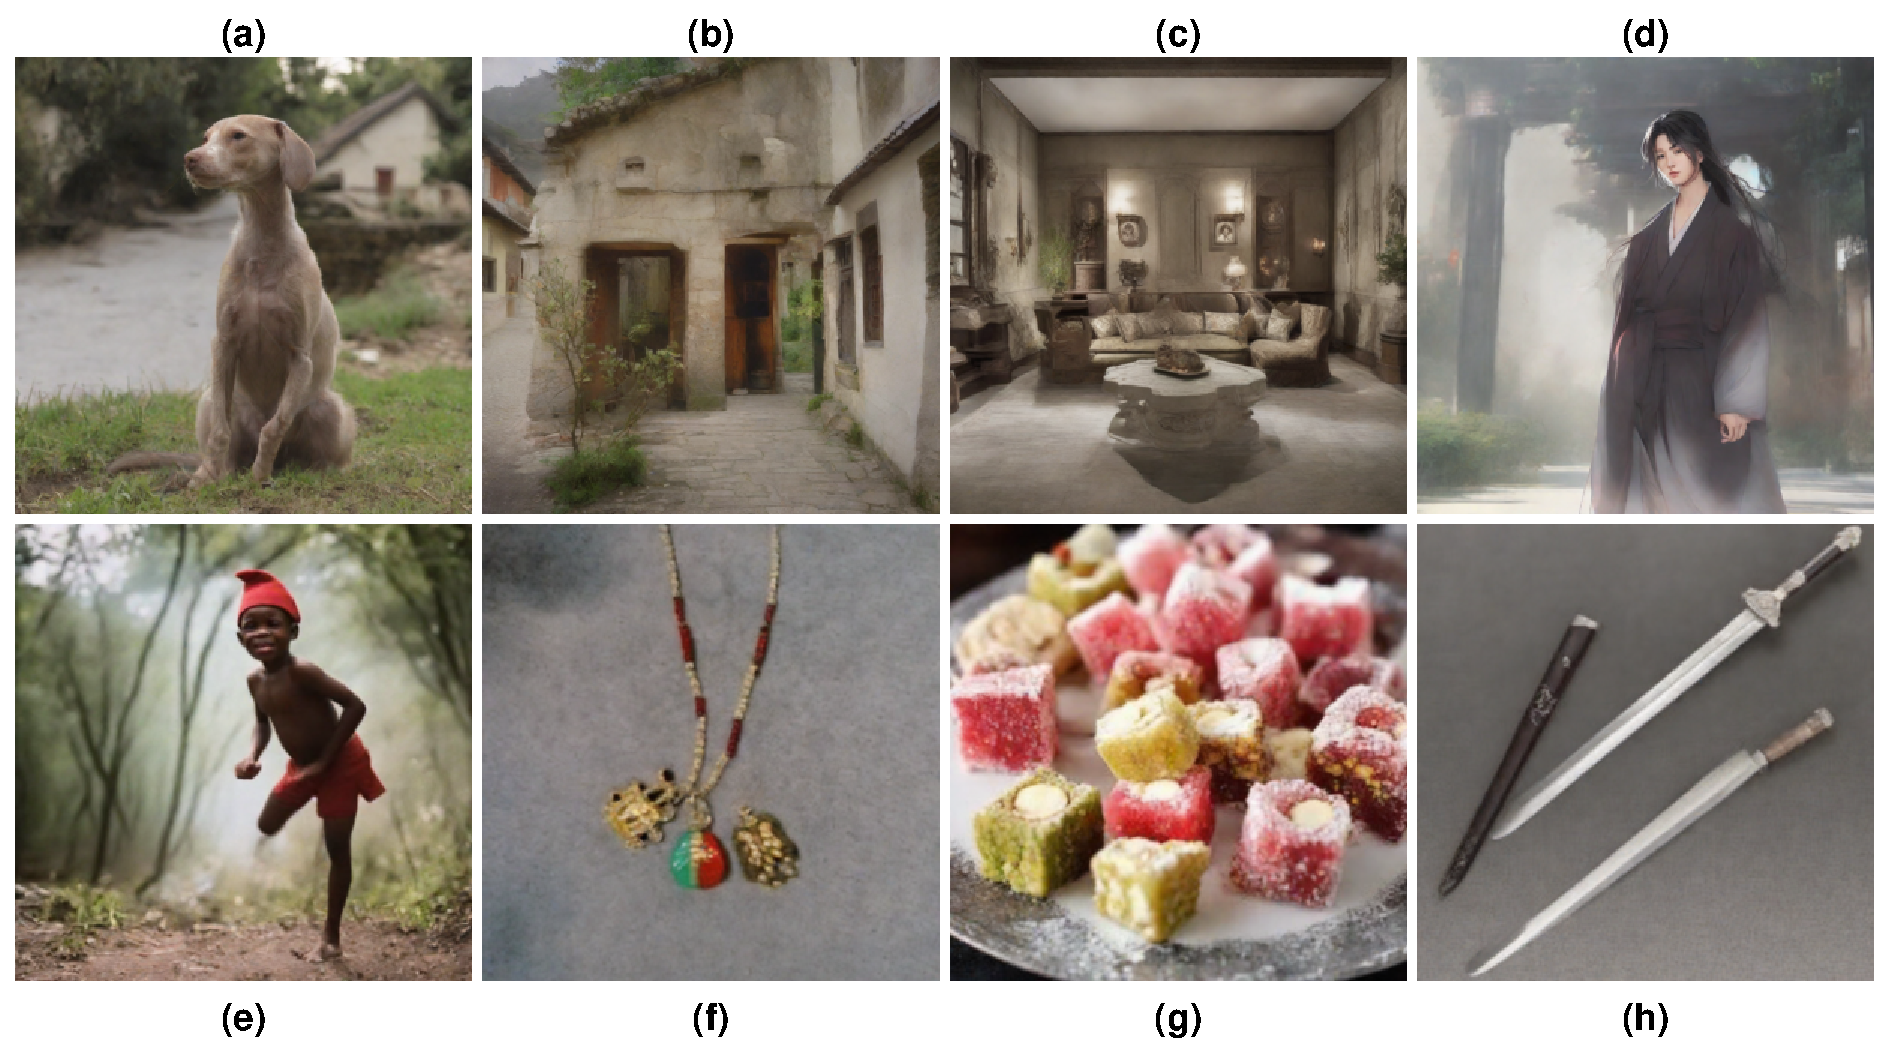
\includegraphics[width=\linewidth]{fig_1_paper.pdf}
    \caption{Generated images before and after training for different concepts\textcolor{blue}{; columns, from left to right, correspond to \textit{Saci}, \textit{Patu\'a}, \textit{Lokum}, and \textit{Jian}}. The top row (a-d) corresponds to images generated by the model before it was introduced to the target concepts. The bottom row (e-h) represents samples generated after training, where the model exhibits improved representations of the intended concepts.}
    \label{fig1}
\end{figure*}


\begin{figure*}[t]
    \centering
    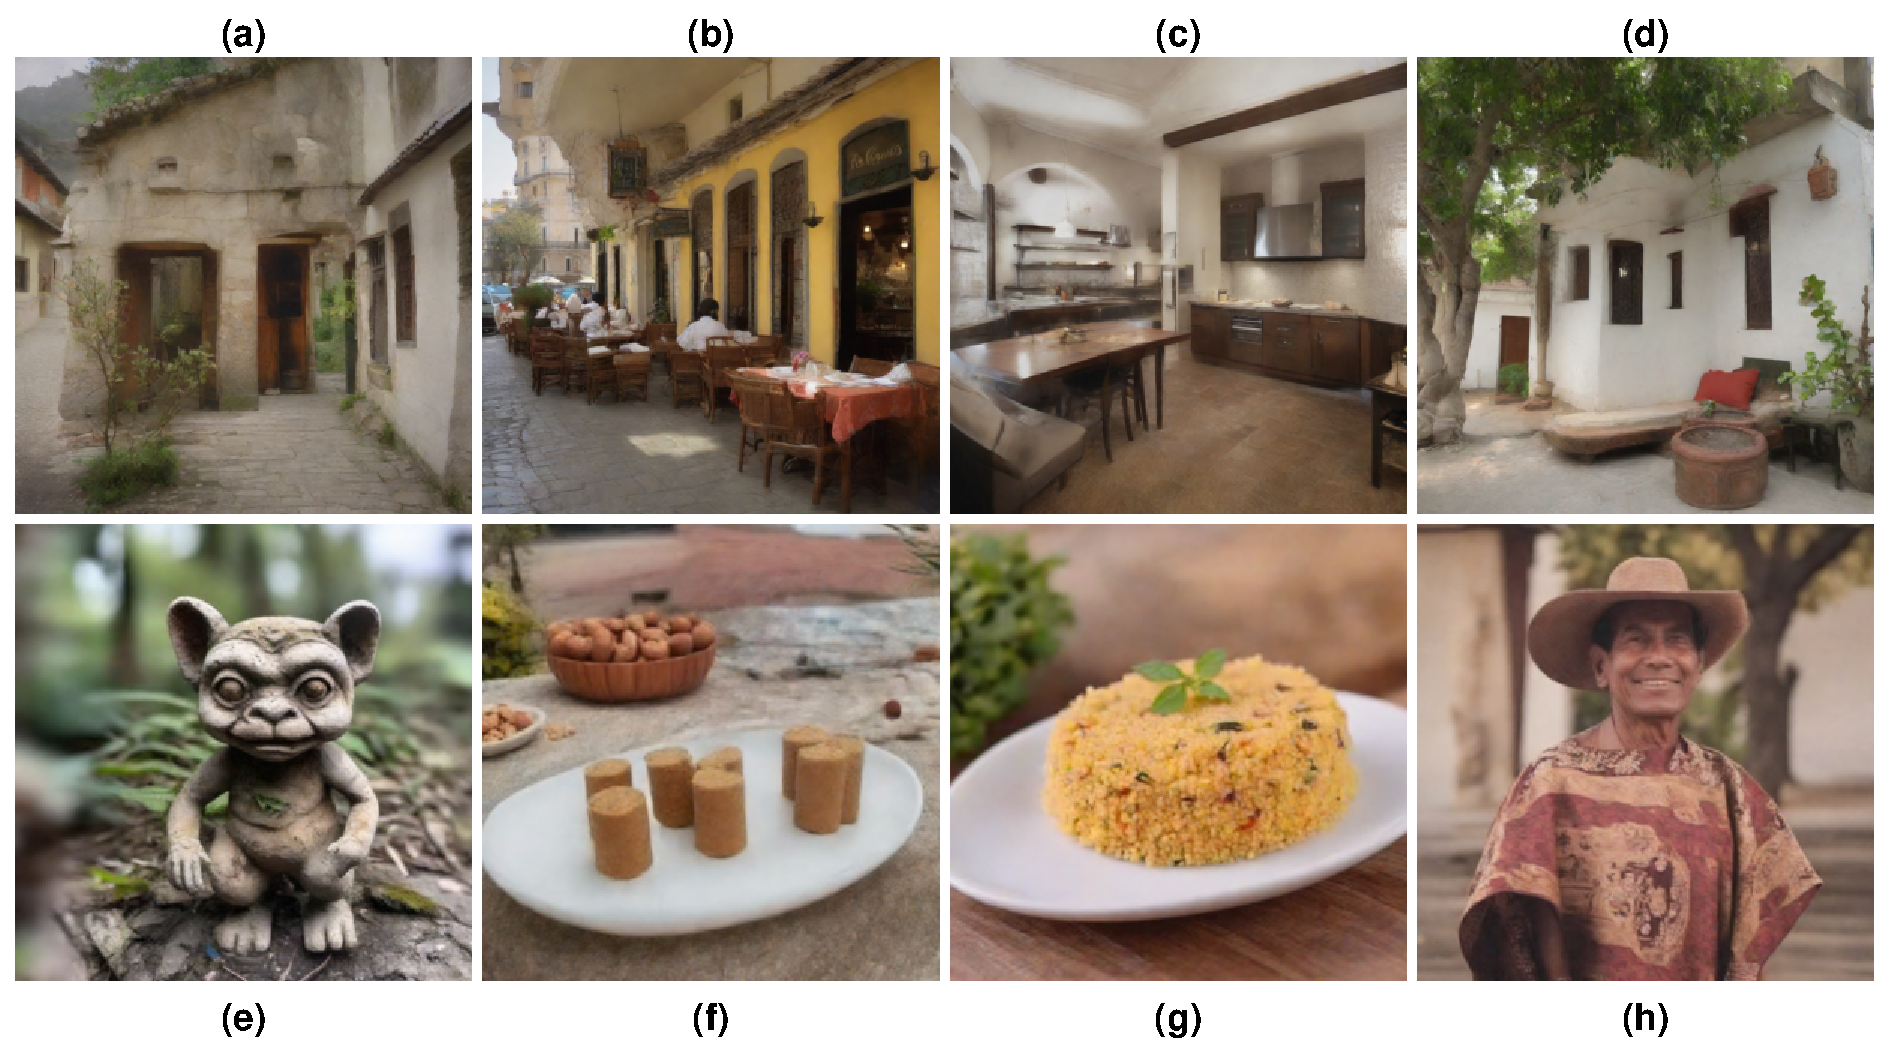
\includegraphics[width=\linewidth]{fig_2_paper.pdf}
    \caption{Additional examples of generated images before and after training\textcolor{blue}{; columns, from left to right, correspond to \textit{Chaneques}, \textit{Pa\c{c}oca}, \textit{Cuscuz}, and \textit{Chamanto}}. Similar to Figure~\ref{fig1}, the top row (a-d) shows pre-training generations, while the bottom row (e-h) presents outputs after concept learning. The figures highlight the impact of model training on the quality and fidelity of the generated images.}
    \label{fig2}
\end{figure*}

It was expected that before training, the model would not have the ability to generate the desired concepts, producing inconsistent images. This aligns with our experimental design, as the selected concepts were chosen precisely because they were unknown to the model. The goal was to teach the model these new concepts and analyze its learning capabilities. Another important aspect of the pre-training images is the observation of potential biases the model may have had regarding these concepts before learning them explicitly. For instance, in Figure~\ref{fig1}(d), although the model hasn't generated a sword, the depiction often included individuals of East Asian descent or artistic styles reminiscent of Chinese culture. This suggests an implicit association between the concept and existing patterns within the model’s training data.

A recurring trend in the pre-training images is the model’s tendency to generate houses or dwellings. This behavior can be observed in $6$ out of the $8$ images presented, suggesting a bias toward architectural structures when encountering unfamiliar concepts. In Figure~\ref{fig1}(e), the model managed to capture several key characteristics of \textit{Saci}, including the red cap, the presence of a single leg, dark skin tone, and a forested background. However, common errors included representations where the character had only one arm or other anatomical deformations. In Figures~\ref{fig1}(f)--(h), the model successfully learned the fundamental essence of the respective concepts. However, a consistent challenge was the accurate depiction of object shapes and textures, with frequent inconsistencies in object connections. Similarly, in Figures~\ref{fig2}(e)--(g), the results indicate successful concept learning, although texture generation remained a challenge. For example, in Figure~\ref{fig2}(f), the model’s representation of \textit{Pa\c{c}oca} appeared grainy due to the brownish color, mistakenly giving it a sandy texture.

Finally, in Figure~\ref{fig2}(h), a notable phenomenon was observed. The training dataset primarily contained images of the Chamanto, a traditional woven garment from central Chile. However, since the dataset did not include many examples of the Chamanto being worn by individuals, the model appears to have misinterpreted its cultural context. Instead, \textcolor{blue}{across the generated samples, it placed the garment in a South Asian visual context: the people, their remaining clothing, and the surroundings resemble Indian imagery, and in a few samples a kumkum (a traditional forehead mark) is visible. Figure~\ref{fig2}(h) shows a representative case, in which the woven garment is worn by a person in a setting unrelated to its Chilean origin. The same tendency is already present before fine-tuning (Figure~\ref{fig2}(d)), which indicates that it originates from the prior of the base model and was not corrected by training images that show the garment almost always on its own, without a human context.} This highlights how training data composition can significantly influence and reinforce cultural biases in generative models, sometimes resulting in incorrect or misleading associations when insufficient contextual information is available.

This result reinforces the importance of maintaining refined manual control over the selection of cultural examples, a task enabled by our Gradio interface. \textcolor{blue}{It also shows that filtering out irrelevant images is not sufficient on its own: all images in the Chamanto training set were verified as depicting the garment, yet few of them showed it being worn in its cultural setting, which left the model free to infer the human context from its own priors. Curation should therefore consider not only the relevance of each image but also the contextual coverage of the set, for instance, by including images of people wearing the garment in its cultural setting. The interface supports this by allowing users to preview the retrieved samples and upload additional images before fine-tuning.} Furthermore, in future work, automated diversity-aware curation solutions—using embedding-space clustering and cultural representativeness metrics~\cite{luccioni2023stablebiasanalyzingsocietal}—can systematically suggest images from different groups and fill cultural gaps, complementing manual curation and strengthening the authenticity of the generated outputs.


The results indicate the success of the proposed methodology in teaching the model new concepts. However, they also emphasize the importance of discussing biases in AI models. Understanding and mitigating these biases is essential to minimize the perpetuation of prejudices, ensuring that AI-generated content is fair and representative. Addressing these concerns is crucial to the responsible development and deployment of AI in society.


\subsection{Quantitative Analysis}

Table~\ref{tab:clip-fid-results} presents a summary of the evaluation outcomes utilizing the CLIP Score and FID metrics for each concept examined. The CLIP Score assesses the semantic similarity between the generated images and \textcolor{blue}{the visual descriptions of the corresponding concepts (Table~\ref{tab:clip_score_prompts})}, with higher scores indicating better alignment. Conversely, the FID metric quantifies the statistical divergence between the distributions of real and generated images, where lower scores denote more desirable results.

\textcolor{blue}{To obtain the numerical results reported here, we substantially increased the sample size relative to our original submission: for each concept, the CLIP Score, FID, and KID were computed individually over $1000$ images generated before fine-tuning and $1000$ images generated after fine-tuning ($3000$ training steps), instead of the $100$ images per condition used previously. This reduces the variance of the metric estimates and yields tighter, more reliable confidence intervals (Table~\ref{tab:clip-fid-results}).} The mean CLIP Score and its standard deviation were then calculated for each concept. In contrast, the FID and KID were computed as statistical distances between the feature distributions of the generated images and those from a reference dataset. The reference dataset consisted of the $20$ real images used to train the model, allowing for a direct comparison of the quality of the generated images against authentic samples.

\begin{table}[htbp]
    \centering
    \caption{\textcolor{blue}{CLIP Score, FID, and KID for each concept, before and after fine-tuning (3000 training steps), computed over 1000 generated images per condition. ``After'' columns report the point estimate and, in brackets, the 95\% bootstrap confidence interval (1000 resamples of the generated images, with the real reference set held fixed); ``Before'' columns report the point estimate only. Higher CLIP Score and lower FID/KID are better. The best post-training value of each metric is shown in bold.}}
    \label{tab:clip-fid-results}
    \fontsize{7}{8.5}\selectfont
    \setlength{\tabcolsep}{2pt}
    \begin{tabular}{@{}lcccccc@{}}
        \toprule
        & \multicolumn{2}{c}{\textbf{CLIP Score} $\uparrow$} & \multicolumn{2}{c}{\textbf{FID} $\downarrow$} & \multicolumn{2}{c}{\textbf{KID} $\downarrow$} \\
        \cmidrule(lr){2-3} \cmidrule(lr){4-5} \cmidrule(l){6-7}
        \textbf{Concept} & \textbf{Before} & \textbf{After} & \textbf{Before} & \textbf{After} & \textbf{Before} & \textbf{After} \\
        \midrule
        \textit{Lokum}      & 17.65 & \textbf{33.12 [32.97, 33.28]} & 330.1 & 229.2 [228.0, 230.9] & 0.121 & 0.069 [0.067, 0.071] \\
        \textit{Pa\c{c}oca} & 16.45 & 25.40 [25.04, 25.74] & 329.4 & 227.7 [223.7, 232.0] & 0.213 & 0.052 [0.048, 0.056] \\
        \textit{Cuscuz}     & 21.38 & 30.18 [30.04, 30.32] & 280.2 & \textbf{177.6 [176.1, 179.5]} & 0.119 & 0.064 [0.062, 0.066] \\
        \textit{Saci}       & 17.64 & 26.60 [26.42, 26.78] & 353.9 & 294.2 [292.3, 296.7] & 0.132 & 0.145 [0.141, 0.148] \\
        \textit{Chaneques}  & 20.47 & 29.91 [29.76, 30.05] & 335.3 & 266.8 [264.9, 269.4] & 0.097 & 0.082 [0.079, 0.085] \\
        \textit{Jian}       & 20.47 & 27.29 [27.04, 27.54] & 360.4 & 240.7 [235.9, 246.5] & 0.209 & 0.065 [0.060, 0.070] \\
        \textit{Chamanto}   & 16.53 & 30.36 [30.13, 30.58] & 365.3 & 204.2 [201.1, 208.0] & 0.160 & \textbf{0.047 [0.045, 0.050]} \\
        \textit{Patu\'a}    & 18.54 & 30.15 [30.03, 30.27] & 354.6 & 218.9 [217.4, 221.1] & 0.166 & 0.062 [0.060, 0.065] \\
        \bottomrule
    \end{tabular}
\end{table}

As observed in Table~\ref{tab:clip-fid-results}, \textcolor{blue}{the post-training results show higher CLIP Scores and lower FID values for all concepts, and lower KID values for seven of the eight concepts, indicating a substantial improvement} in both semantic alignment and image quality. \textcolor{blue}{The exception is \textit{Saci}, whose KID is slightly higher after fine-tuning ($0.145$ vs.\ $0.132$), and whose post-training FID is also the highest among all concepts; \textit{Chaneques}, the other folklore being, shows only a small KID decrease ($0.097$ to $0.082$). Both results are consistent with the higher semantic ambiguity of this category discussed in the group-level analysis below.} \textcolor{blue}{The 95\% confidence intervals are narrow for all three metrics (at most $\pm 0.35$ around the mean for CLIP Score, $\pm 6$ FID points, and $\pm 0.005$ KID) and no post-training interval contains the corresponding before-training value, so both the improvements and the single deterioration (the KID of \textit{Saci}) are larger than the sampling variability of the estimates.} The lower FID and KID scores suggest that the \textcolor{blue}{feature distribution of the model's outputs became closer to that of the real images of each concept}, while the increase in CLIP Score reflects a better match between images and their corresponding textual descriptions.




Among the evaluated concepts, \textit{Lokum} exhibited the highest CLIP Score ($33.12$), indicating that the model was particularly effective in learning this concept from the training dataset. The generated images for \textit{Lokum} closely aligned with \textcolor{blue}{its visual description (Table~\ref{tab:clip_score_prompts})}, demonstrating that the model was able to establish a strong semantic correspondence between image and text. \textit{Cuscuz} exhibited the lowest FID ($177.6$) and \textit{Chamanto} the lowest KID ($0.047$) post-training\textcolor{blue}{; as noted in the qualitative analysis, \textit{Chamanto} is also the concept for which the model most clearly misread the cultural context (associating the garment with an unrelated culture), even though its generated images are, by these two distributional metrics, among the closest to the real training images. This reinforces that low FID/KID values do not guarantee cultural fidelity and that automatic metrics should be complemented with qualitative and, ideally, expert-based assessment.}

\textcolor{blue}{Table~\ref{tab:clip-fid-results} also provides a starting point for group-level comparisons across the three concept categories considered in this study. Aggregating the eight concepts into food (\textit{Cuscuz}, \textit{Lokum}, \textit{Pa\c{c}oca}), folklore beings (\textit{Saci}, \textit{Chaneques}), and artifacts/clothing (\textit{Jian}, \textit{Chamanto}, \textit{Patu\'a}), the post-training CLIP Score is comparable across groups (food: $29.57$, range $[25.40, 33.12]$; folklore beings: $28.25$, range $[26.60, 29.91]$; artifacts/clothing: $29.27$, range $[27.29, 30.36]$), and the same holds for FID (food: $211.6$; folklore beings: $280.5$; artifacts/clothing: $221.3$) and KID (food: $0.062$; folklore beings: $0.113$; artifacts/clothing: $0.058$), with folklore beings showing the largest FID/KID (i.e., the least improvement), driven mainly by \textit{Saci}. Because each group contains only two or three concepts, we report the range (minimum--maximum across concepts) rather than a bootstrap confidence interval, which would not be meaningful at this sample size. Overall, the pipeline does not show a strong systematic advantage or disadvantage for any of the three categories, though the small number of concepts per group limits the strength of this conclusion.}


\begin{figure*}[htbp]
    \centering
    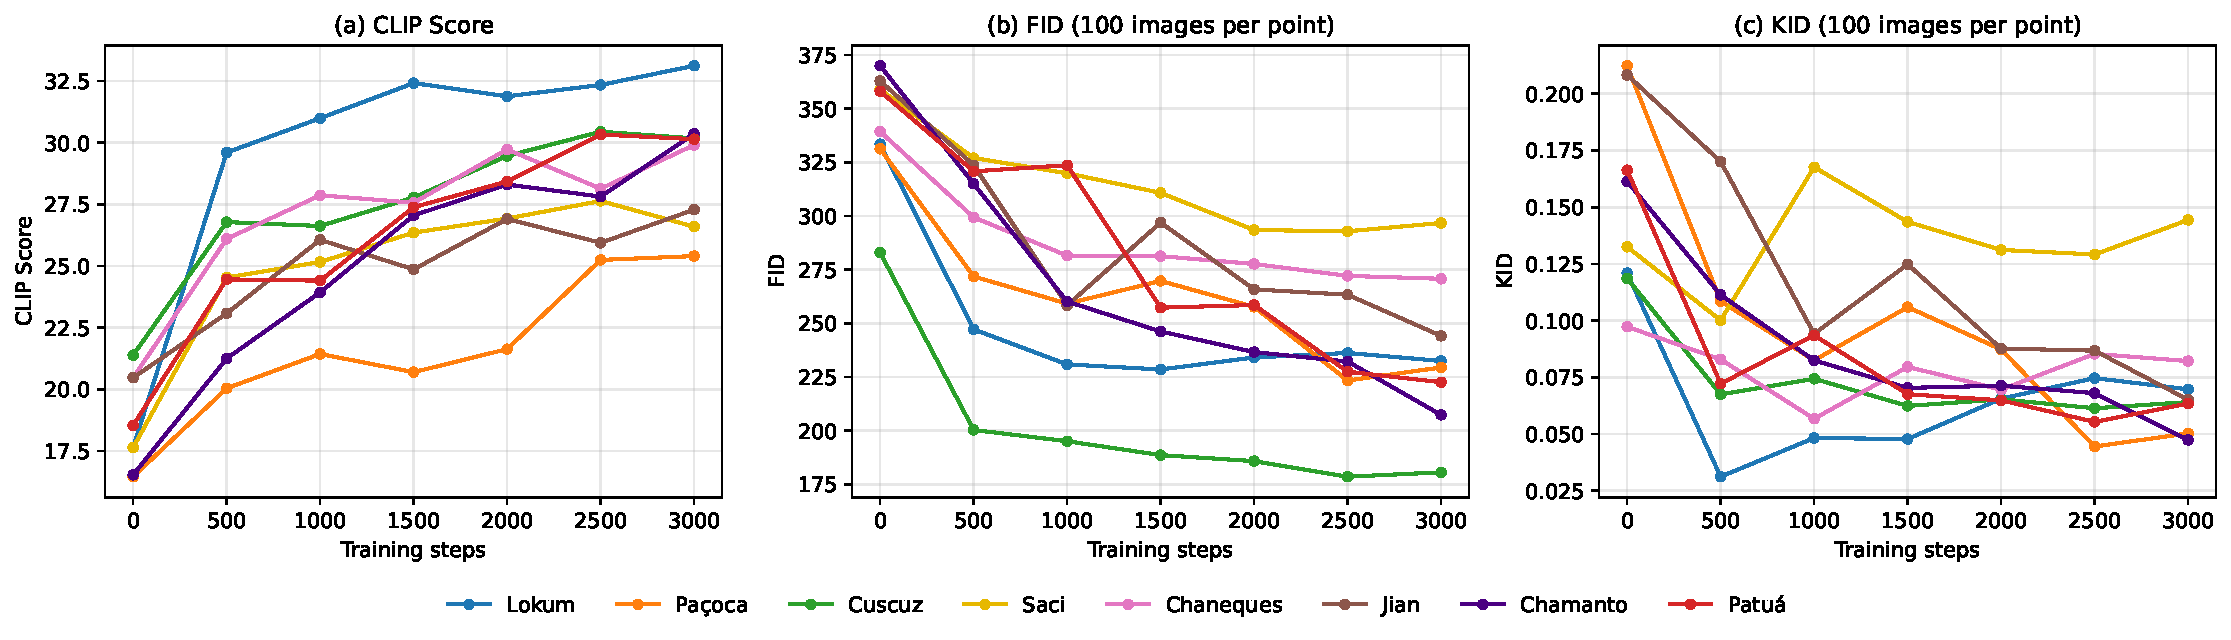
\includegraphics[width=\linewidth]{fig_3_paper.pdf}
    \caption{\textcolor{blue}{Evolution of the three metrics during training. (a) Mean CLIP Score for each concept across training steps, computed on all available images (1000 at steps 0 and 3000, 100 at the intermediate checkpoints); the CLIP Score is a per-image mean and does not depend on the sample size. (b) FID and (c) KID, both computed on 100 images at every point, including steps 0 and 3000, where the value is the average over 50 subsamples of 100 images drawn from the 1000 available; this keeps the points comparable, since FID and KID depend on the number of generated images. The corresponding 1000-image values are reported in Table~\ref{tab:clip-fid-results}.}}
    \label{fig3}
\end{figure*}


To further investigate the fine-tuning process, Figure~\ref{fig3} presents the evolution of \textcolor{blue}{the CLIP Score, FID, and KID} throughout the training process. These results complement the findings in Table~\ref{tab:clip-fid-results}, providing a dynamic view of how the model adapts to new concepts. To conduct this experiment, we performed training checkpoints every $500$ steps, saving intermediate versions of the LoRA fine-tuned models at steps $500$, $1000$, $1500$, $2000$, $2500$, and $3000$. \textcolor{blue}{We generated $1000$ images for the final ($3000$-step) checkpoint of each concept, matching Table~\ref{tab:clip-fid-results}, and $100$ images for each of the five earlier checkpoints ($500$--$2500$ steps). As explained in Section~\ref{methods}, FID and KID are computed here on $100$ images at every point, so that the curve compares like with like; the CLIP Score, being a per-image mean, uses all available images.} To establish a clear comparison baseline, we also included the results of the pre-finetuning model in our analysis. This allowed us to observe how the metrics evolved from the initial model to the final $3000$-step version, providing insights into how the fine-tuning process influenced the quality and semantic accuracy of the generated images over time.

The zero point on the $x$-axis represents the model before fine-tuning, meaning that any improvement in CLIP Score or reduction in FID directly reflects the effectiveness of the adaptation process. As shown in Figure~\ref{fig3}(a), \textcolor{blue}{CLIP Score increases for all concepts within the first $500$ steps, sharply for most of them (e.g., \textit{Lokum} rises from $17.65$ to $29.60$), and continues to rise, with occasional small dips at individual checkpoints, up to the final $3000$-step checkpoint.} This behavior is consistent with the final scores reported in Table~\ref{tab:clip-fid-results}, \textcolor{blue}{where all concepts exhibit a substantial increase in CLIP Score after fine-tuning.} Notably, \textit{Lokum} \textcolor{blue}{stands out with the highest improvement}, suggesting that the model successfully captured its defining characteristics. \textcolor{blue}{Figures~\ref{fig3}(b) and~\ref{fig3}(c) show that FID and KID drop markedly with respect to the base model, indicating that the generated images become more similar to the real samples of each concept, although the decrease is likewise not monotonic across intermediate checkpoints.} This aligns with the FID scores in Table~\ref{tab:clip-fid-results}, where \textit{Cuscuz} achieved the best post-training FID value, highlighting a particularly strong adaptation to this concept.

\textcolor{blue}{The three metrics do not agree on where training should stop. CLIP Score is highest at $3000$ steps for five of the eight concepts (\textit{Lokum}, \textit{Pa\c{c}oca}, \textit{Chaneques}, \textit{Jian}, and \textit{Chamanto}) and at $2500$ steps for the remaining three (\textit{Cuscuz}, \textit{Saci}, and \textit{Patu\'a}), with the $2500$-vs-$3000$ differences for these three being small (at most $1.1$ CLIP Score points). FID is lowest at $3000$ steps for four concepts and at an earlier checkpoint for the other four, by margins of $2.0$ to $6.1$ FID points. KID, which is the most reliable of the three in our small-reference-set regime, is lowest at $3000$ steps for only two concepts (\textit{Jian} and \textit{Chamanto}), at $2500$ for three (\textit{Cuscuz}, \textit{Pa\c{c}oca}, and \textit{Patu\'a}), and as early as $500$--$1000$ steps for \textit{Lokum}, \textit{Saci}, and \textit{Chaneques}; for these last three, the KID at $3000$ steps is $0.025$ to $0.044$ worse than at the best checkpoint, which is a large relative difference.}

\textcolor{blue}{This tension revises the interpretation of our original submission, which attributed the fluctuations after $2000$ steps to overfitting. What the checkpoint-wise evidence supports is narrower: semantic alignment with the target description, as measured by CLIP Score, keeps improving or plateaus until the end of training, whereas the distributional similarity to the real images can degrade after an earlier optimum for some concepts, particularly for \textit{Lokum} and \textit{Saci}. Training for the full $3000$ steps is therefore a reasonable default when the goal is prompt fidelity, but a checkpoint-wise evaluation remains useful, both to select a cheaper model when the computational budget is constrained and to avoid the late-training distributional drift observed for part of the concepts.}

\subsection{\textcolor{blue}{Comparison with Textual Inversion}}
\label{sec:ti-comparison}

\textcolor{blue}{Table~\ref{tab:ti-comparison} compares the fully fine-tuned DreamBooth+LoRA model (checkpoint $3000$) against the Textual Inversion baseline described in Section~\ref{sec:ti-method}, for each concept. DreamBooth+LoRA achieves a higher CLIP Score and a lower FID than Textual Inversion for all eight concepts, by a substantial margin in most cases (mean improvement of $9.0$ CLIP Score points and $115$ FID points). For KID, DreamBooth+LoRA is better for six of the eight concepts; Textual Inversion has a lower KID for \textit{Saci} ($0.131$ vs.\ $0.145$) and \textit{Lokum} ($0.056$ vs.\ $0.069$). None of the $95\%$ confidence intervals of the two methods overlap, for any concept or metric, so these differences, including the two that favor Textual Inversion, are larger than the sampling variability of the estimates. Aggregated by concept group (also Table~\ref{tab:ti-comparison}), DreamBooth+LoRA outperforms Textual Inversion in all three categories in CLIP Score and FID, with the largest gaps for foods ($9.6$ CLIP Score points and $129$ FID points). For KID, it is better for foods and artifacts/clothing, while for folklore beings the two methods are effectively tied ($0.113$ vs.\ $0.115$).}

\textcolor{blue}{One caveat applies to the Textual Inversion column. As discussed at the end of this section, the Textual Inversion embedding drifted toward generating people for several concepts, and part of those images were flagged as not safe for work by an automated classifier and are not part of the released dataset. The Textual Inversion metrics are therefore computed on the images that passed that filter (between $511$ and $987$ of the $1000$ generated per concept, as reported in the last column of Table~\ref{tab:ti-comparison}), whereas the DreamBooth+LoRA metrics use all $1000$ images. Since the removed images are exactly the ones that drifted furthest from the target concept, this filtering favors Textual Inversion; comparing against the unfiltered sets moves its values only slightly and in that direction (e.g., for \textit{Patu\'a}, the concept with the largest number of removed images, unfiltered CLIP Score $19.83$ and KID $0.131$ against filtered $19.96$ and $0.116$), so it does not change any of the comparisons above.}

\begin{table}[htbp]
    \centering
    \caption{\textcolor{blue}{DreamBooth+LoRA (DB) vs.\ Textual Inversion (TI) after fine-tuning/training (1000 generated images per condition). $\Delta$ is DB $-$ TI; negative $\Delta$FID/KID and positive $\Delta$CLIP favor DreamBooth+LoRA. Bottom rows aggregate by concept group.}}
    \label{tab:ti-comparison}
    \fontsize{7}{8.5}\selectfont
    \setlength{\tabcolsep}{2pt}
    \begin{tabular}{@{}lcccccccccc@{}}
        \toprule
        & \multicolumn{3}{c}{\textbf{CLIP Score} $\uparrow$} & \multicolumn{3}{c}{\textbf{FID} $\downarrow$} & \multicolumn{3}{c}{\textbf{KID} $\downarrow$} & \\
        \cmidrule(lr){2-4} \cmidrule(lr){5-7} \cmidrule(lr){8-10}
        & \textbf{DB} & \textbf{TI} & \textbf{$\Delta$} & \textbf{DB} & \textbf{TI} & \textbf{$\Delta$} & \textbf{DB} & \textbf{TI} & \textbf{$\Delta$} & \textbf{TI imgs} \\
        \midrule
        \textit{Chamanto}   & 30.36 & 20.35 & \textbf{+10.01} & 204.2 & 311.8 & \textbf{$-$107.6} & 0.047 & 0.118 & \textbf{$-$0.071} & 960 \\
        \textit{Jian}       & 27.29 & 21.70 & \textbf{+5.58}  & 240.7 & 367.6 & \textbf{$-$126.8} & 0.065 & 0.187 & \textbf{$-$0.122} & 987 \\
        \textit{Patu\'a}    & 30.15 & 19.96 & \textbf{+10.18} & 218.9 & 343.3 & \textbf{$-$124.4} & 0.062 & 0.116 & \textbf{$-$0.054} & 511 \\
        \textit{Chaneques}  & 29.91 & 21.93 & \textbf{+7.98}  & 266.8 & 371.0 & \textbf{$-$104.2} & 0.082 & 0.100 & \textbf{$-$0.018} & 804 \\
        \textit{Saci}       & 26.60 & 17.51 & \textbf{+9.08}  & 294.2 & 363.2 & \textbf{$-$69.1}  & 0.145 & 0.131 & +0.014 & 885 \\
        \textit{Cuscuz}     & 30.18 & 16.23 & \textbf{+13.95} & 177.6 & 366.1 & \textbf{$-$188.5} & 0.064 & 0.183 & \textbf{$-$0.120} & 802 \\
        \textit{Lokum}      & 33.12 & 24.90 & \textbf{+8.22}  & 229.2 & 292.1 & \textbf{$-$63.0}  & 0.069 & 0.056 & +0.013 & 859 \\
        \textit{Pa\c{c}oca} & 25.40 & 18.79 & \textbf{+6.62}  & 227.7 & 361.8 & \textbf{$-$134.1} & 0.052 & 0.163 & \textbf{$-$0.111} & 546 \\
        \midrule
        Food                & 29.57 & 19.97 & \textbf{+9.60}  & 211.5 & 340.0 & \textbf{$-$128.5} & 0.062 & 0.134 & \textbf{$-$0.072} & 736 \\
        Folklore beings     & 28.25 & 19.72 & \textbf{+8.53}  & 280.5 & 367.1 & \textbf{$-$86.6}  & 0.113 & 0.115 & $-$0.002 & 845 \\
        Artifacts/clothing  & 29.27 & 20.67 & \textbf{+8.60}  & 221.3 & 340.9 & \textbf{$-$119.6} & 0.058 & 0.140 & \textbf{$-$0.082} & 819 \\
        \bottomrule
    \end{tabular}
\end{table}

\begin{figure}[htbp]
    \centering
    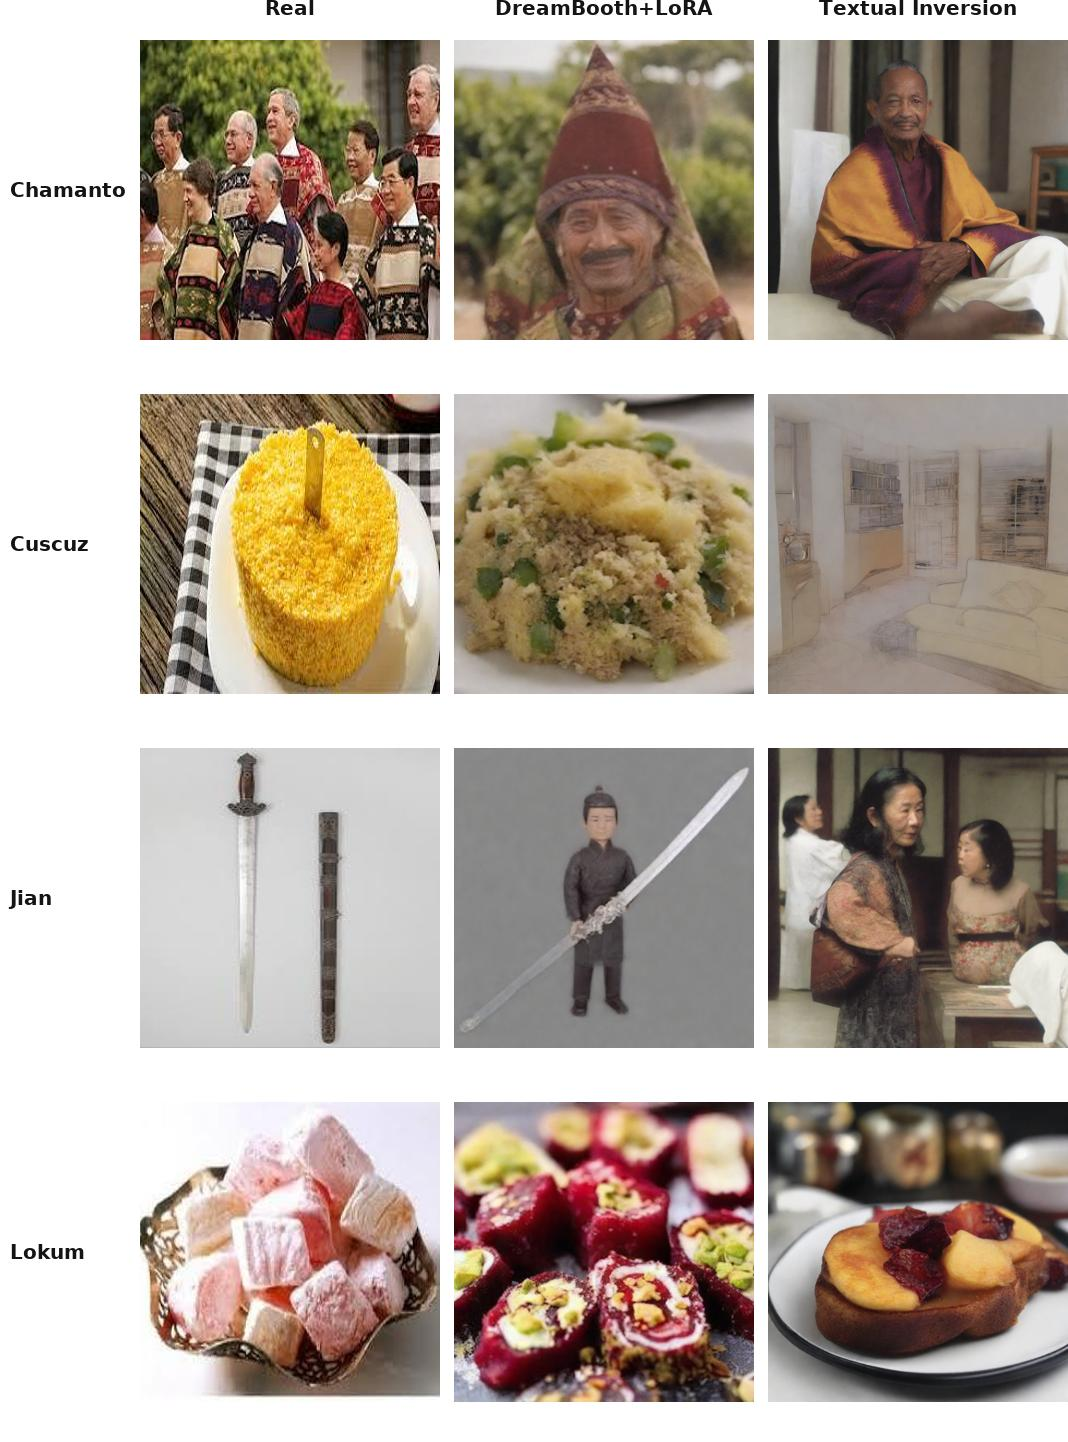
\includegraphics[width=\linewidth]{fig_4_paper.pdf}
    \caption{\textcolor{blue}{Qualitative comparison for four representative concepts: a DreamBooth+LoRA generation and a Textual Inversion generation, both with the same generation settings (LCM, 4 steps, guidance scale 8.0).}}
    \label{fig4}
\end{figure}

\textcolor{blue}{Figure~\ref{fig4} illustrates this gap qualitatively for four representative concepts. DreamBooth+LoRA consistently produces images depicting the target concept, whereas Textual Inversion frequently fails to recover concept-specific visual attributes: for \textit{Chamanto} it generates a person wearing an unrelated shawl, for \textit{Cuscuz} a generic living room with no food at all, and for \textit{Jian} a domestic scene with people rather than a sword. \textit{Lokum} is the case where Textual Inversion comes closest to succeeding, producing a plausible dessert on a plate, though still without the characteristic cubed, sugar-dusted texture of the real product; this is consistent with \textit{Lokum} being one of only two concepts (with \textit{Saci}) for which Textual Inversion obtained a lower KID than DreamBooth+LoRA in Table~\ref{tab:ti-comparison}. We attribute this gap to the difference in capacity between the two methods: LoRA injects and optimizes a set of low-rank matrices throughout the UNet, directly reshaping how the denoising network processes the prompt, whereas Textual Inversion is restricted to finding a single embedding vector that steers the frozen network toward the concept, a much smaller intervention that appears insufficient for most of these visually specific concepts within $3000$ steps. This result should be interpreted as a comparison between our specific configurations of the two methods rather than a general claim about Textual Inversion, since further hyperparameter tuning (e.g., a longer schedule, a category-specific initializer token instead of the generic word ``object'' used in Section~\ref{sec:ti-method}, or a higher learning rate) could narrow this gap. This drift toward unrelated content, frequently toward images of people, also raised a content-safety concern. We screened the Textual Inversion images with the Stable Diffusion safety checker (\texttt{CompVis/stable-diffusion-safety-checker}), which flagged as not safe for work the following numbers of images out of $1000$ per concept: \textit{Patu\'a} $489$, \textit{Pa\c{c}oca} $454$, \textit{Cuscuz} $198$, \textit{Chaneques} $196$, \textit{Lokum} $141$, \textit{Saci} $115$, \textit{Chamanto} $40$, and \textit{Jian} $13$. For DreamBooth+LoRA, the few images flagged by the same checker (for \textit{Chamanto}) were confirmed by manual inspection to be false positives triggered by the fabric and tones of the garment. The flagged images were removed from the publicly released generated-image dataset, and, as noted above, the Textual Inversion metrics in Table~\ref{tab:ti-comparison} are computed on the images that remain. We report this behavior because it is itself a finding about the baseline in this configuration: a personalization method that fails to converge on the target concept does not simply produce neutral images, it can drift toward content that a deployment would have to filter.}

These results highlight the effectiveness of the proposed pipeline in automating the process of creating \texttt{LoRAs} from web-scraped data. \textcolor{blue}{The approach substantially reduces the manual effort involved in dataset collection, annotation, and model training: human intervention is limited to the visual inspection of a small set of images before training. By leveraging this methodology, it is possible to efficiently train models on new concepts, streamlining the process of expanding generative model capabilities.} Furthermore, this technique is particularly valuable for integrating culturally specific concepts into generative models, allowing for the inclusion of diverse local traditions, artifacts, and symbols that might otherwise be underrepresented in large-scale datasets. \textcolor{blue}{By lowering the technical barrier to fine-tuning, this approach could enable local communities to contribute to AI training, fostering a more inclusive and representative development of generative models.}

\subsection{\textcolor{blue}{Practical Guidelines}}
\label{sec:guidelines}

\textcolor{blue}{The experiments above let us extract a set of practical, empirically grounded configuration guidelines for users of the pipeline. These guidelines are derived from the eight concepts studied here and should be read as starting points rather than general rules.}
\begin{itemize}
    \item \textcolor{blue}{\textbf{Dataset size.} About $20$ human-verified images per concept were sufficient to increase the CLIP Score of every concept by at least $6.8$ points (\textit{Jian}) and by up to $15.5$ points (\textit{Lokum}) (Table~\ref{tab:clip-fid-results}).}
    \item \textcolor{blue}{\textbf{Contextual coverage over quantity.} Beyond removing irrelevant images, the set should show the concept in its cultural context (e.g., the garment being worn), since a set of valid but context-poor images led to the cultural misreading observed for \textit{Chamanto} (Section~\ref{results}).}
    \item \textcolor{blue}{\textbf{Training duration.} More than half of the final CLIP Score gain was reached after $1000$ steps for all concepts (between $51\%$ for \textit{Patu\'a} and $86\%$ for \textit{Lokum}), and CLIP Score was highest at $2500$ or $3000$ steps for every concept (Figure~\ref{fig3}). We therefore suggest $3000$ steps as a default and around $1000$ steps when the computational budget is tight. Model selection should not rely on a single metric, however: for three of the eight concepts the KID at $3000$ steps is clearly worse than at an earlier checkpoint, so it is worth evaluating the saved checkpoints rather than assuming the last one is the best.}
    \item \textcolor{blue}{\textbf{Concept category.} Folklore beings, which have fewer canonical depictions, were the hardest category in distributional terms (highest post-training FID and KID, driven by \textit{Saci}); for such concepts, users should favor a larger variety of consistent depictions in the training set.}
    \item \textcolor{blue}{\textbf{Fine-tuning method.} Under matched data and generation settings, DreamBooth+LoRA outperformed Textual Inversion on CLIP Score and FID for every concept, with non-overlapping confidence intervals (Section~\ref{sec:ti-comparison}), so it is the recommended method for visually specific concepts. A method that fails to learn the concept may also drift toward unintended content, which is worth screening for before a deployment.}
    \item \textcolor{blue}{\textbf{Evaluation.} With a reference set of only $20$ real images, absolute FID values are unreliable; CLIP Score against a detailed visual description and KID are better suited for comparing checkpoints, and both should be complemented by visual inspection, since low FID/KID did not prevent the \textit{Chamanto} misreading.}
\end{itemize}

\section{Conclusions}
\label{conclusions}

In this work, we proposed a pipeline for training generative models on previously unknown concepts \textcolor{blue}{using an automated approach with human-guided dataset curation. By leveraging web scraping for dataset collection, visual inspection of the retrieved images, and fine-tuning through LoRAs, we showed that our methodology enables generative models to learn and represent new concepts from approximately twenty images per concept, while reducing manual effort to the inspection of a small number of training samples.} 

\textcolor{blue}{Our evaluation, based on both qualitative and quantitative analyses over 1000 generated images per condition with bootstrap confidence intervals, indicates the effectiveness of the proposed approach across the three concept categories considered in this study (foods, folklore beings, and artifacts). The CLIP Score analysis showed a consistent increase in semantic alignment between generated images and textual descriptions after fine-tuning for all evaluated concepts, while the FID results (for all concepts) and the KID results (for seven of the eight) indicated that the feature distribution of the generated images became closer to that of the real images of each concept. A comparison against a Textual Inversion baseline further showed that DreamBooth+LoRA achieves better CLIP Score and FID for all eight concepts and better KID for six of them, under matched data and generation settings, with no overlap between the confidence intervals of the two methods.} Additionally, the results highlighted the model's tendency to exhibit certain biases depending on the dataset composition, reinforcing the need for careful dataset selection and bias mitigation strategies in generative AI.

Our approach contributes to ongoing discussions on AI development and cultural representation by exploring ways to teach generative models about culturally specific concepts more efficiently. This is particularly relevant for fostering AI systems that are more inclusive and reflective of diverse communities. By examining how local cultural knowledge can be integrated into generative models, we provide insights that may help mitigate biases in large-scale datasets and encourage broader participation in AI development, ultimately contributing to a more culturally aware technology landscape.

\textcolor{blue}{This study also has limitations. First, the quantitative evaluation relies on automatic metrics (CLIP Score, FID, and KID), which are imperfect proxies for cultural fidelity; cultural authenticity was assessed only through the authors' visual inspection, without a formal human evaluation, a user study of the interface, or validation by cultural experts and members of the communities to which the concepts belong. Second, the training images were collected from a single general-purpose source (Google Images) and curated manually, so we did not compare these sets with images from curated cultural repositories. Third, the approach is restricted to tangible visual concepts and to single-modal image generation. Fourth, while we now report bootstrap 95\% confidence intervals for each concept and increased the evaluation sample size from 100 to 1000 generated images per condition, which substantially narrowed these intervals relative to our original submission, our group-level comparisons (food, folklore beings, artifacts/clothing) are based on only two or three concepts per group and are reported as ranges rather than formal statistical tests; a study with more concepts per category would be needed to test for systematic differences between categories with adequate statistical power.}

\textcolor{blue}{Future work could extend data collection to multiple sources, such as open GLAM (galleries, libraries, archives, and museums) collections and curated photo repositories, and explicitly compare web-only and curated training sets. A human evaluation protocol involving cultural experts and members of the corresponding communities, together with a user study of the interface, would provide a more direct assessment of cultural authenticity and usability than automatic metrics alone.} Additionally, \textcolor{blue}{extending the human-in-the-loop design of the Gradio interface from dataset curation to the generated outputs} would empower users to interactively refine the outputs, ensuring stronger alignment with cultural nuances and enhancing the robustness of the generated concepts. Another promising direction is the application of this methodology to other domains beyond image generation, such as video and 3D generative models, broadening the scope of AI applications that benefit from automated knowledge expansion. Moreover, optimizing computational efficiency through adaptive training schedules or early-stopping mechanisms based on real-time metric convergence would make the pipeline even more accessible for resource-constrained settings. Furthermore, incorporating intangible cultural elements—such as traditions, oral narratives, and indigenous symbolism—could further showcase the pipeline’s versatility and deepen its cultural inclusivity. In addition, exploring cross-modal applications—such as linking generated images with culturally grounded text or audio—could lead to richer, multi-sensory representations of heritage, opening new paths for educational, artistic, and preservation-oriented use cases. Overall, our results demonstrate the potential of an automated pipeline for fine-tuning generative models, offering a powerful tool for expanding AI capabilities while promoting diversity and cultural inclusivity in generative AI systems.


\section{Declarations}

\subsection*{Availability of data and material}
\textcolor{blue}{The code of the pipeline (image scraping, training, generation, and evaluation) and the metric results supporting the findings of this study are publicly available at \url{https://github.com/Fmahlow/Auto-Tune}. The full set of generated images used for the evaluation in this revision (DreamBooth+LoRA and Textual Inversion, all concepts and checkpoints), together with the trained LoRA weights and Textual Inversion embeddings, is publicly available at \url{https://huggingface.co/datasets/FelipeMahlow/auto-tune-generated-images}. The training images were collected from Google Images and may be protected by third-party copyright, so they are not redistributed; they can be collected again with the provided scraping code and the concept names in Table~\ref{tab:clip_score_prompts}, although search results may change over time.}

\subsection*{Competing interests}
The authors have no competing interests to declare that are relevant to the content of this article.

\subsection*{Funding}
This work is supported by Coordena\c{c}{\~a}o de Aperfei\c{c}oamento de Pessoal de N{\'i}vel Superior (CAPES), projects number 88887.607339/2021-00, 88887.192403/2025-00  and Funda\c{c}{\~a}o de Amparo {\`a} Pesquisa do Estado de S{\~a}o Paulo (FAPESP), grant Nos. 2023/12830-0 and 2024/14934-0.

\subsection*{Authors' contributions}
Felipe Mahlow led the conceptualization, methodology design, pipeline implementation, and writing of the manuscript. Renato Dias de Souza contributed to system integration, dataset collection, and experimental evaluation. João Paulo Papa supervised the research and contributed to \textcolor{blue}{the experimental design.} Kelton Augusto Pontara da Costa provided technical oversight and contributed to the design of the web-based interface and computational infrastructure. All authors read and approved the final manuscript.

\subsection*{Acknowledgements}
The authors would like to thank the São Paulo State University (UNESP) for the research infrastructure support. Additional thanks to the Hugging Face and Gradio communities for providing open-source tools used in this work.


\bibliography{references}
%% if required, the content of .bbl file can be included here once bbl is generated
%%\input sn-article.bbl

\end{document}
